%************************************************
\section{Session tracking}\label{p02:session_tracking}
%************************************************

In order to understand the learning process, we need to keep track of the working sessions. The term refers to either reading or exercising sessions. A reading session is considered as an uninterrupted reading activity of a particular article, while an exercise session can encompass multiple articles. Given the fact that students can switch between windows or even walk away from the screen, a method to compute the effective working time is devised. 

\subsection{Algorithm}
Working sessions are computed under the assumption that all user actions fall into one out of three types: opening, interaction or closing events.

Depending on the type of event, a working session can be either created, updated (kept alive) or finalized. With this simple approach, the algorithm can be fine tuned by adding or removing events (\eg, including the scrolling as a interaction event).

Additionally, there is a \textbf{session\_timeout} parameter which is used to handle scenarios where a session was not properly closed. In these cases, the session is closed and a bonus of \textbf{session\_timeout} minutes are added to the last action date and time, under the assumption that the user did not stop working immediately after the last action.

Typical scenarios are:

\begin{itemize}
	\item When the browser was closed or the computer was turned off.
	
	\item When the user is inactive for a long period.
	
	\item When the user is taking unusually too long between actions the activity is considered as suspicious.
\end{itemize}


\begin{figure}[bth]
	{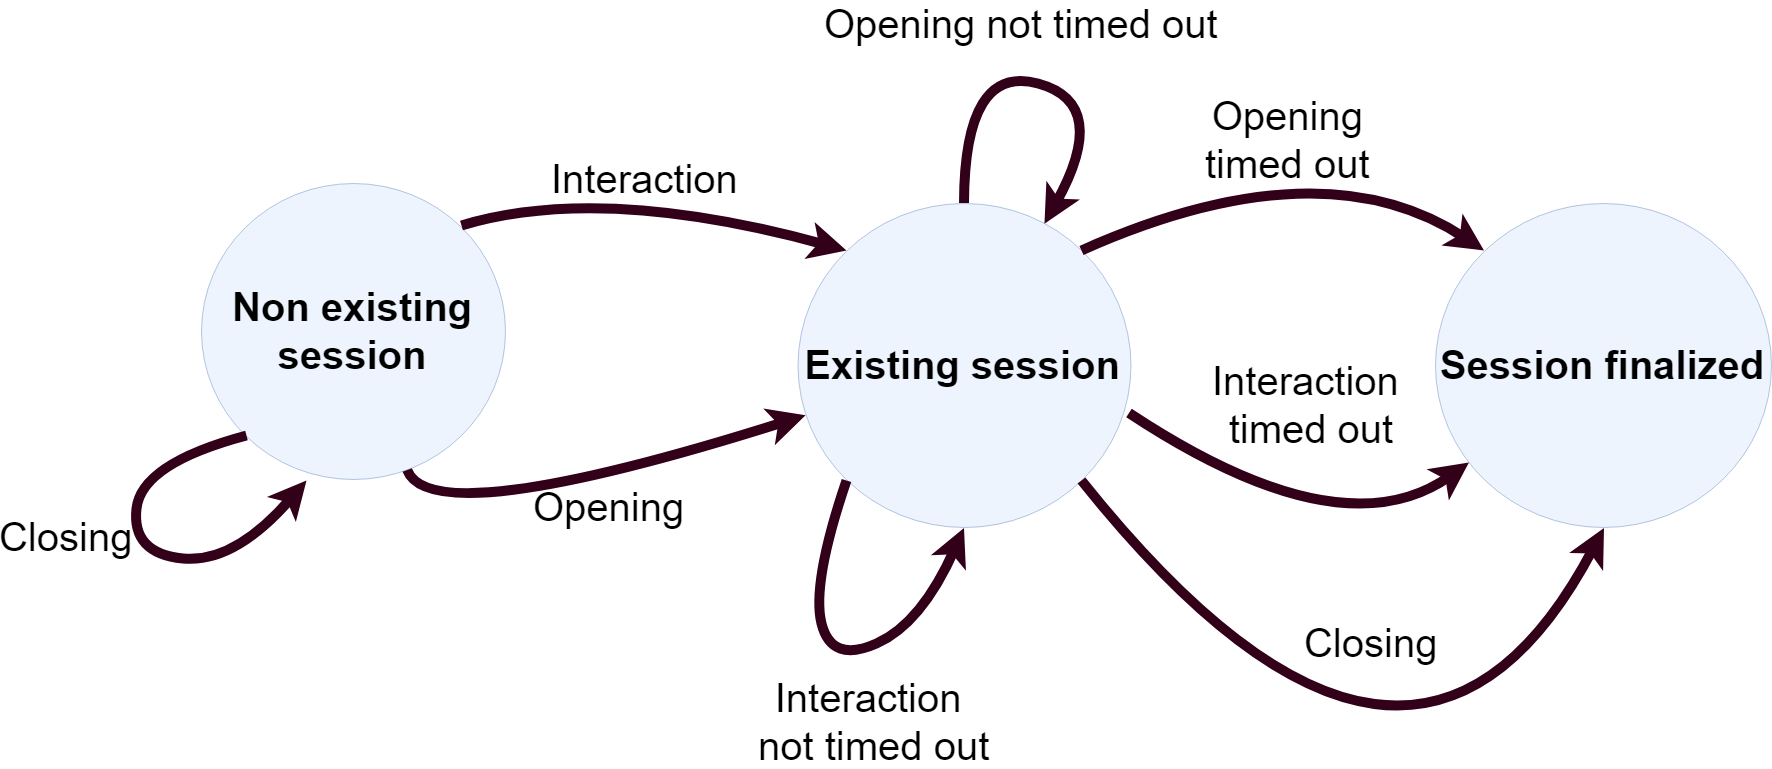
\includegraphics[width=1\linewidth]{gfx/Finite_state_machine_diagramv2}} \quad
	\caption[Finite state diagram - Working session transitions due to user actions]{Finite state diagram - Working session transitions due to user actions}\label{fig:markov_diagram}
\end{figure}

Figure \ref{fig:markov_diagram} depicts the life span of a working session.
The circles represent the three states in which a session can be:
\begin{itemize}
	\item Non existing session: this is the initial status, this means there is no active session for the user within the current context (\Ie\ no active reading session for the current article and user, or not active exercise session for the user). 
	\item Existing session: if there is already an existing/active session in the same context, the session falls in the second status.
	\item Session finalized: the moment that the session is closed due to a timeout or the user performing a closing action. After this status, no further actions can modify the session.
\end{itemize}

The arrows represent the type of user actions that trigger the change of status of the session:
\begin{itemize}
	\item Opening: actions that mark the beginning of a working session, such as beginning to read or to exercise.
	\item Opening timed out: opening actions that happen after the timeout has expired, this can lead to a different status.
	\item Opening not timed out: opening actions that happen before the timeout is expired.
	\item Interaction: most of user actions fall within this category, they are the actions that imply the student is actively working.
	\item Interaction timed out: interaction actions that happen after the timeout is expired
	\item Interaction not timed out: interaction actions that occur before the timeout is reached
	\item Closing: when the user manually finalizes the current activity.
\end{itemize}


\subsection{Architecture}
For the specific case of Zeeguu platform, the implementation of the algorithm is divided in two layers: front and back ends. The front end is implemented in Javascript and it tracks the user actions with the system. The back end is implemented in Python and is where the logic for the working sessions is implemented.

Figure \ref{fig:session_tracking_architecture} shows the architecture of the solution. The implementation is divided in two layers, which can work independently. 

Relevant user actions are detected by the front end layer of the system, and stored in the database. The back end periodically retrieves the list of user events and stitches them to extend the session or creates a new session depending on the type of event and the time between the actions. Therefore inserting the session information back in the database, making it available to be displayed.
The front end layer can also trigger the execution of the session stitching module after each user activity, enabling real time session analysis.
Event stitching is the process of creating or expanding a session between two consecutive user actions.

%TODO include layers diagram
\begin{figure}[bth]
	\centering
	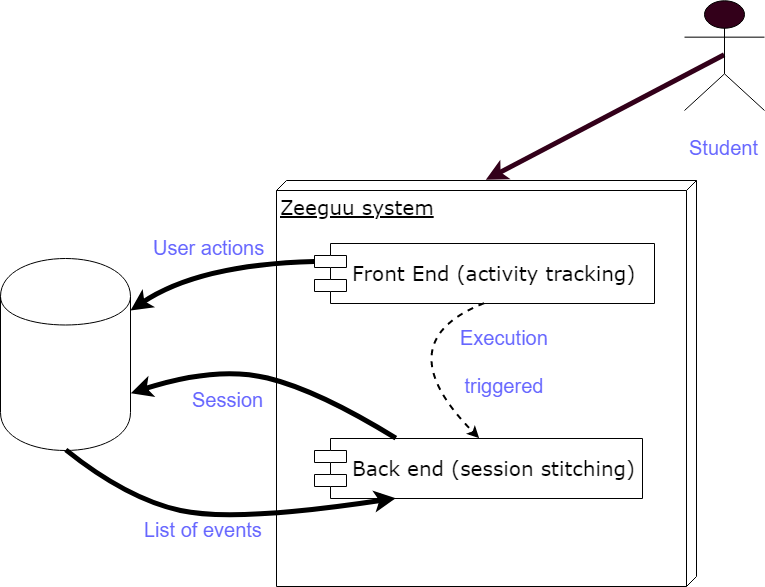
\includegraphics[width=0.7\linewidth]{gfx/session_tracking_architecture}
	\caption{Session tracking architecture}\label{fig:session_tracking_architecture}
\end{figure}

\subsection{Reading session}\label{p02:session_tracking_read_session}
For the reading session, Javascript listeners are used to track the following user events:
\begin{itemize}
	\item Open list of articles
	\item Open an article
	\item Translate a word
	\item Undo a word translation
	\item Lose and gain focus on the page
	\item Scrolling
	\item Close an article
\end{itemize}

When these events are detected, the related information is immediately stored in the database. Each time the back end runs, it stitches the events to the corresponding session, until the article is closed or a new article is opened. In which case, the back end finalizes the session, making it available to be visualized.

While defining what a session is in the system, and given the fact that the application is on the web, the following difficulties are encountered:
\begin{itemize}
	\item Events like closing the browser or turning off the computer cannot be detected
	\item If the user walks away from the screen, we cannot detect exactly when it was and if he read a couple of minutes before leaving
	\item The user can open multiple instances of Zeeguu, and each instance can have a different article open
	\item If the user opened multipe articles, the user can change from article to article in a short time period
	\item The user can be using more than one device at the same time
	\item The user can read an article in multiple sessions
\end{itemize}

Therefore the following assumptions for the implementation of the reading session are considered:
\begin{itemize}
\item Reading sessions are considered per article. Therefore, when the user opens a new article we consider it as a new session. In this way we solve the issue where the same user could have opened different articles in different tabs and switches between them.

\item For scenarios when the user leaves the session open for a time period longer than the session\_timeout, we give it a time benefit of “session\_timeout” minutes, because we cannot know exactly how long after the last action, the user kept reading. 

\item A user can read the same article multiple times, and each time is considered a new session.
\end{itemize}

As mentioned before, a timeout parameter is used for finalizing a session after \textbf{N} number of minutes. If the timeout value is too small an advanced student that does not translate any word but reads a long text might be incorrectly measured, while if the value is too big, we would incorrectly consider longer reading sessions. Therefore, defining the value of the timeout is crucial. 


\subsection{Exercise session}
For the exercise sessions, the front end layer starts a timer when the exercise is opened. When it is answered (either correct or incorrect) or a hint is requested, the event is stored in the database with the elapsed time.

The back end layer is immediately executed after the front end code, appending the recently answered exercise to the exercise session or creating a new one when the elapsed time is larger than the timeout value.

Therefore, opening an exercise does not count for the active session, only answering.

For exercise sessions, the algorithm can be more precise on the tracking because an exercise usually comes surrounded by a single sentence, therefore the timeout can be set to a smaller value. 

The final difference with the reading session is that no "benefit time" is granted to the user, the only actions that keep the session alive are answering the exercise.


%TODO explain events tracked and events that were added

%TODO explain script for historical data


%TODO Later, the implementation of the algorithm in the system, for this, it was needed to implement additional user actions detection (lost focus, and scrolling)